\begin{table}
\small\centering
\begin{tabular}{@{}lll@{}}
\toprule
{\bf Pattern }    & { }  & {\bf Strip Mined Pattern} \\ \midrule
{\begin{lstlisting}[mathescape=true,numbers=none,basicstyle=\fontsize{8}{8}\selectfont\tt]
T[ Map(d)(m) ]
\end{lstlisting}
} & \texttt{=} &
{\begin{lstlisting}[mathescape=true,numbers=none,basicstyle=\fontsize{8}{8}\selectfont\tt]
MultiFold(d/b)(d)(zeros(d)){ i =>
  (i, acc => Map(b)(T[m]) )
}(_)
\end{lstlisting}
} \\ \midrule
{\begin{lstlisting}[mathescape=true,numbers=none,basicstyle=\fontsize{8}{8}\selectfont\tt]
T[ MultiFold(d)(r)(z)(g)(c) ]
\end{lstlisting}
} & \texttt{=} &
{\begin{lstlisting}[mathescape=true,numbers=none,basicstyle=\fontsize{8}{8}\selectfont\tt]
MultiFold(d/b)(r)(T[z]){ i =>
  (i, acc => T[c](acc, MultiFold(b)(r)(T[z])(T[g])(T[c])) )
}(T[c])
\end{lstlisting}
} \\ \midrule
{\begin{lstlisting}[mathescape=true,numbers=none,basicstyle=\fontsize{8}{8}\selectfont\tt]
T[ GroupByFold(d)(z)(h)(c) ]
\end{lstlisting}
} & \texttt{=} &
{\begin{lstlisting}[mathescape=true,numbers=none,basicstyle=\fontsize{8}{8}\selectfont\tt]
GroupByFold(d/b)(T[z]){ i =>
  GroupByFold(b)(T[z])(T[h])(T[c])
}(T[c])
\end{lstlisting}
} \\ \midrule
{\begin{lstlisting}[mathescape=true,numbers=none,basicstyle=\fontsize{8}{8}\selectfont\tt]
T[ FlatMap(d)(f) ]
\end{lstlisting}
} & \texttt{=} &
{\begin{lstlisting}[mathescape=true,numbers=none,basicstyle=\fontsize{8}{8}\selectfont\tt]
FlatMap(d/b){i => FlatMap(b)(T[f]) }
\end{lstlisting}
} \\ \bottomrule
\end{tabular}
\caption{Strip mining transformation rules for parallel patterns defined in Figure \ref{fig:ppl-syntax}.}
\label{table:stripmining}
\end{table}


\section{Strip Mining}
\label{sec:strip-mining}
We first examine how parallel patterns can be strip mined.
In imperative programs, \emph{for} loops are strip mined using a single transformation
rule: split the loop's domain to create a pair of nested \emph{for} loops.
The rules for parallel pattern strip mining are similarly straightforward
but pattern-specific.

The strip mining algorithm is defined here using two passes over the IR.
The first pass partitions each pattern's iteration domain \emph{d} into tiles of
size \emph{b} by breaking the pattern into a pair of perfectly nested patterns.
The outer pattern operates over the strided index domain, expressed here as
\emph{d/b}, while the inner pattern operates on a tile of size \emph{b}.
For the sake of brevity this notation ignores the case where \emph{b} does not
perfectly divide \emph{d}, but this case is solved in practice with the
addition of bounds checks on the domain of the inner loop.

Table~\ref{table:stripmining} gives an overview of the rules used by the transformer
(denoted $T$) to strip mine parallel patterns.
In addition to splitting up the domain, patterns are transformed by recursively
strip mining all functions within that pattern.
Map is strip mined by reducing its domain and range and nesting it within a MultiFold.
Note that the strided MultiFold writes to each memory location only once.
In this case, we indicate the MultiFold's combination function as unused with an underscore.

As defined in Figure~\ref{fig:ppl-syntax}, the MultiFold, GroupByFold, and FlatMap patterns have the property that a perfectly nested form of a single instance of one of these
patterns is equivalent to a single ``flattened'' form of that same pattern. This property allows these patterns to be strip mined by
breaking them up into a set of perfectly nested patterns of the same type as the original pattern.

The second strip mining pass converts array slices and accesses with statically predictable access patterns into slices and accesses of larger, explicitly defined
array memory tiles. We define tiles which have a size statically known to fit on the FPGA using array copies.
Copies generated during strip mining will be used to infer buffers during hardware generation.
These buffers in turn will allow better usage of burst reads and writes from main memory and enable overlapping of compututation and communication using hardware prefetching.
Array tiles which have overlap, such as those generated from sliding windows in convolution, are marked with metadata in the IR as having some reuse factor.
Array copies with reuse have generation rules which minimize the number of redundant reads to main memory when possible.

\begin{table}
\small\centering
\begin{tabular}{@{}lll@{}}
\toprule
{\bf High Level Language}                            & {\bf PPL }       & {\bf Strip Mined PPL} \\ \midrule
{\begin{lstlisting}[language=Scala,numbers=none,backgroundcolor=\color{white}]
// Element-wise Map
val x = Array[Float](d)
x.map{e => 2*e}
\end{lstlisting}}
&
{\begin{lstlisting}[language=PPLTable,numbers=none,basicstyle=\fontsize{7}{7}\beramonott,backgroundcolor=\color{white},backgroundcolor=\color{white}]
map(d){i => 2*x(i)}
\end{lstlisting}}
&
{\begin{lstlisting}[language=PPLTable,numbers=none,basicstyle=\fontsize{7}{7}\beramonott,backgroundcolor=\color{white}]
multiFold(d/b)(d)(zeros(d)){ii =>
  xTile = x.copy(b + ii)
  (i, map(b)(b){i => 2*xTile(i) })
}(_)
\end{lstlisting}} \\ \midrule
{\begin{lstlisting}[language=Scala,numbers=none,basicstyle=\fontsize{7}{7}\beramonott,backgroundcolor=\color{white}]
// Sums along matrix rows
val x = Array2D[Float](m x n)
x.map{ row =>
  row.fold(0){ (a,b) => a + b }
}
\end{lstlisting}}
&
{\begin{lstlisting}[language=PPLTable,numbers=none,basicstyle=\fontsize{7}{7}\beramonott,backgroundcolor=\color{white}]
multiFold(m,n)(m)(zeros(m))
{ (i,j) =>
  (i, acc => acc + x(i,j))
}{(a,b) =>
  map(n){(j) => a(j) + b(j)}
}
\end{lstlisting}}
&
{\begin{lstlisting}[language=PPLTable,numbers=none,basicstyle=\fontsize{7}{7}\beramonott,backgroundcolor=\color{white}]
multiFold(m/b0,n/b1)(m)(zeros(m)){ (ii,jj) =>
  xTile = x.copy(b0 + ii, b1 + jj)
  tile = multiFold(b0,b1)(b0)(zeros(b0)){ (i,j) =>
    (i, acc => acc + xTile(i,j))
  }{(a,b) => map(b0){i => a(i) + b(i)} }
  (ii, acc => map(b0){j => acc(j) + tile(j)})
}{(a,b) =>
  multiFold(m/b0)(m)(zeros(m)){ii =>
    aTile = a.copy(b0 + ii)
    bTile = a.copy(b0 + ii)
    (ii, acc => map(b0){i => aTile(i) + bTile(i)})
  }{(a,b) => map(m){i => a(i) + b(i)}}
}
\end{lstlisting}} \\ \midrule
{\begin{lstlisting}[language=Scala,numbers=none,basicstyle=\fontsize{7}{7}\beramonott,backgroundcolor=\color{white}]
// Simple Filter
val x = Array[Float](d)
x.flatMap{ e =>
  if (e > 0) e else []
}
\end{lstlisting}}
&
{\begin{lstlisting}[language=PPLTable,numbers=none,basicstyle=\fontsize{7}{7}\beramonott,backgroundcolor=\color{white}]
flatMap(d){i =>
  if (x(i) > 0) x(i) else []
}
\end{lstlisting}}
&
{\begin{lstlisting}[language=PPLTable,numbers=none,basicstyle=\fontsize{7}{7}\beramonott,backgroundcolor=\color{white}]
flatMap(d/b)(1){ii =>
  eTile = x.copy(b + ii)
  flatMap(b){i =>
    if (eTile(i) > 0) eTile(i) else []
}}
\end{lstlisting}} \\ \midrule
{\begin{lstlisting}[language=Scala,numbers=none,basicstyle=\fontsize{7}{7}\beramonott,backgroundcolor=\color{white}]
// Histogram Calculation
val x = Array[Float](d)
x.groupByFold(0){ r =>
  (r/10, 1)
}{ (a,b) => a + b }
\end{lstlisting}}
&
{\begin{lstlisting}[language=PPLTable,numbers=none,basicstyle=\fontsize{7}{7}\beramonott,backgroundcolor=\color{white}]
groupByFold(d)(0){i =>
  (x(i)/10, 1)
}{(a,b) => a + b }
\end{lstlisting}}
&
{\begin{lstlisting}[language=PPLTable,numbers=none,basicstyle=\fontsize{7}{7}\beramonott,backgroundcolor=\color{white}]
groupByFold(d/b)(0){ii =>
  xTile = x.copy(b + ii)
  groupByFold(b)(0){i =>
    (xTile(i)/10, 1)
  }{(a,b) => a + b}
}{(a,b) => a + b}
\end{lstlisting}} \\ \bottomrule
\end{tabular}
\caption{Examples of the parallel pattern strip mining transformation on Map, MultiFold, FlatMap, and GroupByFold}
\label{table:stripmine-examples}
\end{table}


Table~\ref{table:stripmine-examples} demonstrates how our rules can be used to strip mine a set of simple data parallel operations.
We use the \emph{copy} infix function on arrays to designate array copies in these examples, using similar syntax as array \emph{slice}.
We assume in these examples that common subexpression elimination (CSE) and code motion transformation passes have been run after strip mining to eliminate duplicate copies and to
move array tiles out of the innermost patterns. In these examples, strip mining creates tiled copies of input collections that
we can later directly use to infer read buffers.

\section{Pattern Interchange}

\begin{figure}
\centering

\begin{lstlisting}[language=Scala,numbers=none,basicstyle=\fontsize{9}{10}\beramonott]
// Matrix Multiplication
x: Array[Array[Float]] // m x p
y: Array[Array[Float]] // p x n
z = x.map{row =>
  y.map{col =>
    row.zipWith(col){(a,b) =>
      a * b
    }.sum
  }
}
\end{lstlisting}
a. High level language for matrix multiplication of matrices x and y.
\vspace{10pt}

\begin{lstlisting}[language=Scala,numbers=none,basicstyle=\fontsize{9}{10}\beramonott]
multiFold(m/b0,n/b1)(m,n)(zeros(m,n)){(ii,jj) =>
(*@\color{vbgray}{\vrule}@*)  ((ii,jj), zTile =>
(*@\color{vbgray}{\vrule}@*)  (*@\color{vbgray}{\vrule}@*)  map(b0,b1){(i,j) =>
(*@\color{vbgray}{\vrule}@*)  (*@\color{vbgray}{\vrule}@*)  (*@\color{vbgray}{\vrule}@*)  tile = multiFold(p/b2)(1)(0){ kk =>
(*@\color{vbgray}{\vrule}@*)  (*@\color{vbgray}{\vrule}@*)  (*@\color{vbgray}{\vrule}@*)  (*@\color{vbgray}{\vrule}@*)  xTile = x.copy(b0 + ii, b2 + kk)
(*@\color{vbgray}{\vrule}@*)  (*@\color{vbgray}{\vrule}@*)  (*@\color{vbgray}{\vrule}@*)  (*@\color{vbgray}{\vrule}@*)  yTile = y.copy(b2 + kk, b1 + jj)
(*@\color{vbgray}{\vrule}@*)  (*@\color{vbgray}{\vrule}@*)  (*@\color{vbgray}{\vrule}@*)  (*@\color{vbgray}{\vrule}@*)  dprod = fold(b2)(0){ k =>
(*@\color{vbgray}{\vrule}@*)  (*@\color{vbgray}{\vrule}@*)  (*@\color{vbgray}{\vrule}@*)  (*@\color{vbgray}{\vrule}@*)  (*@\color{vbgray}{\vrule}@*)  acc => acc + xTile(i,k) * yTile(k,j)
(*@\color{vbgray}{\vrule}@*)  (*@\color{vbgray}{\vrule}@*)  (*@\color{vbgray}{\vrule}@*)  (*@\color{vbgray}{\vrule}@*)  }{(a,b) => a + b})
(*@\color{vbgray}{\vrule}@*)  (*@\color{vbgray}{\vrule}@*)  (*@\color{vbgray}{\vrule}@*)  (*@\color{vbgray}{\vrule}@*)  (0, elemTile => elemTile + dprod)
(*@\color{vbgray}{\vrule}@*)  (*@\color{vbgray}{\vrule}@*)  (*@\color{vbgray}{\vrule}@*)  }{(a,b) => a + b}
(*@\color{vbgray}{\vrule}@*)  (*@\color{vbgray}{\vrule}@*)  (*@\color{vbgray}{\vrule}@*)  zTile(i,j) + tile
(*@\color{vbgray}{\vrule}@*)  })
}(_)
\end{lstlisting}
b. Strip mined PPL representation.
\vspace{10pt}

\begin{lstlisting}[language=Scala,numbers=none,basicstyle=\fontsize{9}{10}\beramonott]
multiFold(m/b0,n/b1)(m,n)(zeros(m,n)){(ii,jj) =>
(*@\color{vbgray}{\vrule}@*)  tile = multiFold(p/b2)(b0,b1)(...){kk =>
(*@\color{vbgray}{\vrule}@*)  (*@\color{vbgray}{\vrule}@*)  xTile = x.copy(b0 + ii, b2 + kk)
(*@\color{vbgray}{\vrule}@*)  (*@\color{vbgray}{\vrule}@*)  yTile = y.copy(b2 + kk, b1 + jj)
(*@\color{vbgray}{\vrule}@*)  (*@\color{vbgray}{\vrule}@*)  (0, elemTile =>
(*@\color{vbgray}{\vrule}@*)  (*@\color{vbgray}{\vrule}@*)  (*@\color{vbgray}{\vrule}@*)  map(b0,b1){(i,j) =>
(*@\color{vbgray}{\vrule}@*)  (*@\color{vbgray}{\vrule}@*)  (*@\color{vbgray}{\vrule}@*)  (*@\color{vbgray}{\vrule}@*)  dprod = fold(b2)(0){ k =>
(*@\color{vbgray}{\vrule}@*)  (*@\color{vbgray}{\vrule}@*)  (*@\color{vbgray}{\vrule}@*)  (*@\color{vbgray}{\vrule}@*)  (*@\color{vbgray}{\vrule}@*)  acc => acc + xTile(i,j) * yTile(j,k)
(*@\color{vbgray}{\vrule}@*)  (*@\color{vbgray}{\vrule}@*)  (*@\color{vbgray}{\vrule}@*)  (*@\color{vbgray}{\vrule}@*)  }{(a,b) => a + b}
(*@\color{vbgray}{\vrule}@*)  (*@\color{vbgray}{\vrule}@*)  (*@\color{vbgray}{\vrule}@*)  (*@\color{vbgray}{\vrule}@*)  elemTile(i,j) + dprod
(*@\color{vbgray}{\vrule}@*)  (*@\color{vbgray}{\vrule}@*)  })
(*@\color{vbgray}{\vrule}@*)  }{(a,b) =>
(*@\color{vbgray}{\vrule}@*)  (*@\color{vbgray}{\vrule}@*)  map(b0,b1){(i,j) => a(i,j) + b(i,j)
(*@\color{vbgray}{\vrule}@*)  }
(*@\color{vbgray}{\vrule}@*)  ((ii,jj), zTile =>
(*@\color{vbgray}{\vrule}@*)  (*@\color{vbgray}{\vrule}@*)  map(b0,b1){(i,j) => zTile(i,j) + tile(i,j)}
(*@\color{vbgray}{\vrule}@*)  })
}(_)
\end{lstlisting}
c. Interchanged PPL representation.

\caption{Example of the pattern interchange transformation applied to matrix multiplication.}
\label{fig:interchange-examples}
\end{figure}


Given an intermediate representation with strip mined nested parallel patterns, we now need to interchange patterns to increase the reuse
of newly created data tiles. This can be achieved by moving strided patterns out of unstrided patterns. However, as with imperative loops,
it is not sound to arbitrarily change the order of nested parallel patterns.
We adapt two rules for pattern interchange from a previously established \emph{Collect}-\emph{Reduce} reordering rule for computation on clusters~\cite{brown16clusters}.
These rules both match on the special case of MultiFold where every iteration updates the entire accumulator, which we refer to here as a \emph{fold}.
The first interchange rule defines how to move a scalar, strided \emph{fold} out of an unstrided Map, transforming the nested loop into a strided \emph{fold} of a Map.
Note that this also changes the combination function of the \emph{fold} into a Map.
The second rule is the inverse of the first, allowing us to reorder a strided MultiFold with no reduction function (i.e. the outer pattern of a tiled Map)
out of an unstrided \emph{fold}. This creates a strided MultiFold of a scalar \emph{fold}. We apply these two rules whenever possible to increase the reuse
of tiled inputs.

Imperfectly nested parallel patterns commonly occur either due to the way the original user program was structured or
as a result of aggressive vertical fusion run prior to tiling.
Interchange on imperfectly nested patterns requires splitting patterns into perfectly nested sections. However, splitting and reordering trades
temporal locality of intermediate values for increased reuse of data tiles. In hardware, this can involve creating more main memory
reads or larger on-chip buffers for intermediate results so that less reads need to be done for input and output data. This tradeoff between memory reads and
increased buffer usage requires more complex cost modeling.
We use a simple heuristic to determine whether to split fused loops: we split and interchange patterns only when
the intermediate result created after splitting and interchanging is statically known to fit on the FPGA. This handles the simple case
where the FPGA has unused on-chip buffers and allocating more on-chip memory guarantees a decrease in the number of main memory reads.

Figure~\ref{fig:interchange-examples} shows a simple example of the application of our pattern interchange rules on matrix multiplication.
We assume here that loop invariant code motion has been run again after pattern interchange has completed.
In matrix multiplication, we interchange the perfectly nested strided MultiFold and the unstrided Map.
This ordering increases the reuse of the copied tile of matrix \emph{y} and changes the scalar reduction into a tile-wise reduction.
Note that the partial result calculation and the inner reduction can now be vertically fused.

\section{Coarse-Grained Pipelining}
To generate high performance hardware from parallel patterns, it is insufficient
to exploit only a single level of parallelism. Exploiting nested parallelism
requires mechanisms to orchestrate the flow of data through multiple pipeline
stages while also exploiting parallelism at each stage of execution.
The end result are pipelined loops which are themselves pipelined with other
pipelined loops and memory controllers, resulting in a hierarchy of pipelines,
commonly referred to as a coarse-grained pipeline (or occassionally, ``metapipeline'').

Most FPGA-specific control scheduling is done by the lower level compiler as described in Chapter~\ref{scheduling}. However, unlike the lower level Spatial compiler, the higher level
compiler operates on parallel patterns which have inherent parallelism information.
We therefore perform a simple pipeline schedule analysis in the high level compiler
so that the Spatial compiler is able to perform pipelining scheduling without
also having to re-derive this parallelism information.

Pipeline scheduling is done as a recursive traversal of the hierarchical IR.
At each level, we create pipeline schedules by first performing a topological sort on the IR
of the body of the current parallel pattern. The result is a list of stages,
where each stage contains a list of patterns which can be run concurrently.
Exploiting the pattern's semantic information, we then
optimize the pipeline schedule by removing unnecessary memory transfers and redundant computation.
For instance, if the output memory region of the pattern has been assigned to an array marked as a buffer,
we do not generate unnecessary writes to main memory.

Our functional representation of tiled parallel patterns
can sometimes create redundant accumulation functions, for example, in cases where a MultiFold is tiled into a nested MultiFold. During scheduling we identify
this redundancy and emit a single copy of the accumulator, removing the unnecessary intermediate buffer.
Finally, in cases where the accumulator of a MultiFold cannot completely fit on-chip, we add a special
forwarding path between the stages containing the accumulator. This optimization avoids redundant writes to memory and
reuses the current tile.
Once we have the final pipeline schedule for a parallel pattern,
we mark the parallel pattern as a pipeline candidate and save the
schedule as metadata for later use by the lower level Spatial compiler.

\section{Example}

\begin{figure}\small\centering
\hspace{-0.105\textwidth}
\centering\begin{tabular}{cm{0.45\textwidth}m{0.01\textwidth}m{0.44\textwidth}}
{} &
{\begin{lstlisting}
(sums,counts) = multiFold(n/b0)((k,d),k)(...){ii =>
(*@\color{vbgray}{\vrule}@*)  pt1Tile = points.copy(b0 + ii, *)
(*@\color{vbgray}{\vrule}@*)
(*@\color{vbgray}{\vrule}@*)  multiFold(b0)((k,d),k)(zeros(1,d),0){ i =>
(*@\color{vbgray}{\vrule}@*)  (*@\color{vbgray}{\vrule}@*)  pt1 = pt1Tile.slice(i, *)
(*@\color{vbgray}{\vrule}@*)  (*@\color{vbgray}{\vrule}@*)  minDistWithIndex = multiFold(k/b1)(1)((max, -1)){ jj =>
(*@\color{vbgray}{\vrule}@*)  (*@\color{vbgray}{\vrule}@*)  (*@\color{vbgray}{\vrule}@*)  pt2Tile = centroids.copy(b1 + jj, *)
(*@\color{vbgray}{\vrule}@*)  (*@\color{vbgray}{\vrule}@*)  (*@\color{vbgray}{\vrule}@*)  minIndTile = fold(b1)((max,-1)){ j =>
(*@\color{vbgray}{\vrule}@*)  (*@\color{vbgray}{\vrule}@*)  (*@\color{vbgray}{\vrule}@*)  (*@\color{vbgray}{\vrule}@*)  pt2 = pt2Tile.slice(j, *)
(*@\color{vbgray}{\vrule}@*)  (*@\color{vbgray}{\vrule}@*)  (*@\color{vbgray}{\vrule}@*)  (*@\color{vbgray}{\vrule}@*)  dist = distance(pt1, pt2)
(*@\color{vbgray}{\vrule}@*)  (*@\color{vbgray}{\vrule}@*)  (*@\color{vbgray}{\vrule}@*)  (*@\color{vbgray}{\vrule}@*)  acc => if (acc._1 < dist) acc else (dist, j+jj)
(*@\color{vbgray}{\vrule}@*)  (*@\color{vbgray}{\vrule}@*)  (*@\color{vbgray}{\vrule}@*)  }{ (a,b) => if (a._1 < b._1) a else b }
(*@\color{vbgray}{\vrule}@*)  (*@\color{vbgray}{\vrule}@*)  (*@\color{vbgray}{\vrule}@*)
(*@\color{vbgray}{\vrule}@*)  (*@\color{vbgray}{\vrule}@*)  (*@\color{vbgray}{\vrule}@*)  (0, {acc =>
(*@\color{vbgray}{\vrule}@*)  (*@\color{vbgray}{\vrule}@*)  (*@\color{vbgray}{\vrule}@*)    if (acc._1 < minIndTile._1) acc
(*@\color{vbgray}{\vrule}@*)  (*@\color{vbgray}{\vrule}@*)  (*@\color{vbgray}{\vrule}@*)    else minIndTile
(*@\color{vbgray}{\vrule}@*)  (*@\color{vbgray}{\vrule}@*)  (*@\color{vbgray}{\vrule}@*)  })
(*@\color{vbgray}{\vrule}@*)  (*@\color{vbgray}{\vrule}@*)  }{(a,b) =>
(*@\color{vbgray}{\vrule}@*)  (*@\color{vbgray}{\vrule}@*)    if (a._1 < b._1) a else b
(*@\color{vbgray}{\vrule}@*)  (*@\color{vbgray}{\vrule}@*)  }
(*@\color{vbgray}{\vrule}@*)  (*@\color{vbgray}{\vrule}@*)
(*@\color{vbgray}{\vrule}@*)  (*@\color{vbgray}{\vrule}@*)
(*@\color{vbgray}{\vrule}@*)  (*@\color{vbgray}{\vrule}@*)  minDistIndex = minDistWithIndex._2
(*@\color{vbgray}{\vrule}@*)  (*@\color{vbgray}{\vrule}@*)  sumFunc = ... // Fig 4: lines 17-20
(*@\color{vbgray}{\vrule}@*)  (*@\color{vbgray}{\vrule}@*)  countFunc = ... // Fig 4: line 21
(*@\color{vbgray}{\vrule}@*)  (*@\color{vbgray}{\vrule}@*)  (sumFunc, countFunc)
(*@\color{vbgray}{\vrule}@*)  }{(a,b) => ... /* Tiled combination function */ }
(*@\color{vbgray}{\vrule}@*)  (0, acc => ... /* Tiled combination function */ )
}{(a,b) => ... /* Tiled combination function */ }
}
\end{lstlisting}} & \hfill &
%\end{minipage} \hfill
%\begin{minipage}[b]{.4\textwidth}
{\begin{lstlisting}
(sums,counts) = multiFold(n/b0)((k,d),k)(...){ ii =>
(*@\color{vbgray}{\vrule}@*)  pt1Tile = points.copy(b0 + ii, *)
(*@\color{vbgray}{\vrule}@*)  minDistWithInds =
(*@\color{vbgray}{\vrule}@*)    multiFold(k/b1)(b1)(map(b1)((max, -1))){ jj =>
(*@\color{vbgray}{\vrule}@*)  (*@\color{vbgray}{\vrule}@*)  pt2Tile = centroids.copy(b1 + jj, *)
(*@\color{vbgray}{\vrule}@*)  (*@\color{vbgray}{\vrule}@*)  minIndsTile = map(b0){ i =>
(*@\color{vbgray}{\vrule}@*)  (*@\color{vbgray}{\vrule}@*)  (*@\color{vbgray}{\vrule}@*)  pt1 = pt1Tile.slice(i, *)
(*@\color{vbgray}{\vrule}@*)  (*@\color{vbgray}{\vrule}@*)  (*@\color{vbgray}{\vrule}@*)  minIndTile = fold(b1)((max,-1)){ j =>
(*@\color{vbgray}{\vrule}@*)  (*@\color{vbgray}{\vrule}@*)  (*@\color{vbgray}{\vrule}@*)  (*@\color{vbgray}{\vrule}@*)  pt2 = pt2Tile.slice(j, *)
(*@\color{vbgray}{\vrule}@*)  (*@\color{vbgray}{\vrule}@*)  (*@\color{vbgray}{\vrule}@*)  (*@\color{vbgray}{\vrule}@*)  dist = distance(pt1, pt2)
(*@\color{vbgray}{\vrule}@*)  (*@\color{vbgray}{\vrule}@*)  (*@\color{vbgray}{\vrule}@*)  (*@\color{vbgray}{\vrule}@*)  acc => if (acc._1 < dist) acc else (dist, j+jj)
(*@\color{vbgray}{\vrule}@*)  (*@\color{vbgray}{\vrule}@*)  (*@\color{vbgray}{\vrule}@*)  }{ (a,b) => if (a._1 < b._1) a else b }
(*@\color{vbgray}{\vrule}@*)  (*@\color{vbgray}{\vrule}@*)  }
(*@\color{vbgray}{\vrule}@*)  (*@\color{vbgray}{\vrule}@*)  (0, acc => map(b0){ i =>
(*@\color{vbgray}{\vrule}@*)  (*@\color{vbgray}{\vrule}@*)    if (acc(i)._1 < minIndsTile(i)._1) acc
(*@\color{vbgray}{\vrule}@*)  (*@\color{vbgray}{\vrule}@*)    else minIndsTile(i)
(*@\color{vbgray}{\vrule}@*)  (*@\color{vbgray}{\vrule}@*)  })
(*@\color{vbgray}{\vrule}@*)  }{(a,b) =>
(*@\color{vbgray}{\vrule}@*)    map(b0){i => if (a(i)._1 < b(i)._1) a(i) else b(i) }
(*@\color{vbgray}{\vrule}@*)  }
(*@\color{vbgray}{\vrule}@*)  multiFold(b0)(k,d)(zeros(k,d)){ i =>
(*@\color{vbgray}{\vrule}@*)  (*@\color{vbgray}{\vrule}@*)  pt1 = pt1Tile.slice(i, *)
(*@\color{vbgray}{\vrule}@*)  (*@\color{vbgray}{\vrule}@*)  minDistIndex = minDistWithInds(i)._2
(*@\color{vbgray}{\vrule}@*)  (*@\color{vbgray}{\vrule}@*)  sumFunc = ... // Fig 4: lines 17-20
(*@\color{vbgray}{\vrule}@*)  (*@\color{vbgray}{\vrule}@*)  countFunc = ... // Fig 4: line 21
(*@\color{vbgray}{\vrule}@*)  (*@\color{vbgray}{\vrule}@*)  (sumFunc, countFunc)
(*@\color{vbgray}{\vrule}@*)  }{(a,b) => ... /* Tiled combination function */ }
(*@\color{vbgray}{\vrule}@*)  (0, acc => ... /* Tiled combination function */ )
}{(a,b) => ... /* Tiled combination function */ }
}
\end{lstlisting}}
\end{tabular}

\vspace{-0.2in}\begin{tabular}{cc}
{\parbox{0.45\textwidth}{\centering{a. Strip mined $k$-means in PPL.}}} &
{\parbox{0.5\textwidth}{\centering{b. Pattern interchanged $k$-means in PPL.}}}
\end{tabular}

%\vspace{-0.045\textwidth}
\hspace{-0.180\textwidth}
\centering\begin{tabular}{cm{0.45\textwidth}m{0.01\textwidth}m{0.44\textwidth}}
{} &
{\begin{lstlisting}[numbers=none,language=Pseudo]
1     For each tile of b0 points:
2     (*@\color{vbgray}{\vrule}@*)  Copy the points tile into local memory
3 - 4 (*@\color{vbgray}{\vrule}@*)  (*@\textbf{\color{blue}{For each point \emph{pt1} in the points tile}}@*):
5     (*@\color{vbgray}{\vrule}@*)  (*@\color{vbgray}{\vrule}@*)  (*@\textbf{\color{red}{For each tile of b1 centroids}}@*):
6     (*@\color{vbgray}{\vrule}@*)  (*@\color{vbgray}{\vrule}@*)  (*@\color{vbgray}{\vrule}@*)  Copy the centroids tile into local memory
7 - 8 (*@\color{vbgray}{\vrule}@*)  (*@\color{vbgray}{\vrule}@*)  (*@\color{vbgray}{\vrule}@*)  For each centroid (*@\emph{pt2}@*) in the centroids tile:
9     (*@\color{vbgray}{\vrule}@*)  (*@\color{vbgray}{\vrule}@*)  (*@\color{vbgray}{\vrule}@*)  (*@\color{vbgray}{\vrule}@*)  Compute distance between (*@\emph{pt1}@*) and (*@\emph{pt2}@*)
10-11 (*@\color{vbgray}{\vrule}@*)  (*@\color{vbgray}{\vrule}@*)  (*@\color{vbgray}{\vrule}@*)  (*@\color{vbgray}{\vrule}@*)  Keep the closest (index,distance) pair
      (*@\color{vbgray}{\vrule}@*)  (*@\color{vbgray}{\vrule}@*)  (*@\color{vbgray}{\vrule}@*)  End
13-16 (*@\color{vbgray}{\vrule}@*)  (*@\color{vbgray}{\vrule}@*)  (*@\color{vbgray}{\vrule}@*)  Keep the closest pair across tiles
      (*@\color{vbgray}{\vrule}@*)  (*@\color{vbgray}{\vrule}@*)  End
20    (*@\color{vbgray}{\vrule}@*)  (*@\color{vbgray}{\vrule}@*)  Extract the index of the closest centroid
21    (*@\color{vbgray}{\vrule}@*)  (*@\color{vbgray}{\vrule}@*)  Add (*@\emph{pt1}@*) to row minDistIndex
22    (*@\color{vbgray}{\vrule}@*)  (*@\color{vbgray}{\vrule}@*)  Increment count at minDistIndex
24    (*@\color{vbgray}{\vrule}@*)  (*@\color{vbgray}{\vrule}@*)  Add point and count sums across tiles
      (*@\color{vbgray}{\vrule}@*)  End
25-26 (*@\color{vbgray}{\vrule}@*)  Add point and count sums across tiles
      End
\end{lstlisting}} & \hfill &
%\end{minipage} \hfill
%\begin{minipage}[b]{.4\textwidth}
{\begin{lstlisting}[numbers=none,language=Pseudo]
1     For each tile of b0 points:
2     (*@\color{vbgray}{\vrule}@*)  Copy the points tile into local memory
3     (*@\color{vbgray}{\vrule}@*)  (*@\color{red}{\textbf{For each tile of b1 centroids}}@*):
4     (*@\color{vbgray}{\vrule}@*)  (*@\color{vbgray}{\vrule}@*)  Copy the centroids tile into local memory
5 - 6 (*@\color{vbgray}{\vrule}@*)  (*@\color{vbgray}{\vrule}@*)  (*@\color{blue}{\textbf{For~each~point~\emph{pt1}~in~the~points~tile:}}@*)
7 - 8 (*@\color{vbgray}{\vrule}@*)  (*@\color{vbgray}{\vrule}@*)  (*@\color{vbgray}{\vrule}@*)  For each centroid (*@\emph{pt2}@*) in the centroids tile:
9     (*@\color{vbgray}{\vrule}@*)  (*@\color{vbgray}{\vrule}@*)  (*@\color{vbgray}{\vrule}@*)  (*@\color{vbgray}{\vrule}@*)  Compute distance between (*@\emph{pt1}@*) and (*@\emph{pt2}@*)
10-11 (*@\color{vbgray}{\vrule}@*)  (*@\color{vbgray}{\vrule}@*)  (*@\color{vbgray}{\vrule}@*)  (*@\color{vbgray}{\vrule}@*)  Keep the closest (index,distance) pair
      (*@\color{vbgray}{\vrule}@*)  (*@\color{vbgray}{\vrule}@*)  (*@\color{vbgray}{\vrule}@*)  End
      (*@\color{vbgray}{\vrule}@*)  (*@\color{vbgray}{\vrule}@*)  End
13-16 (*@\color{vbgray}{\vrule}@*)  (*@\color{vbgray}{\vrule}@*)  For each point: keep the closest pair across tiles
      (*@\color{vbgray}{\vrule}@*)  End
18-19 (*@\color{vbgray}{\vrule}@*)  (*@\color{blue}{\textbf{For each point \emph{pt1} in points tile}}@*):
20    (*@\color{vbgray}{\vrule}@*)  (*@\color{vbgray}{\vrule}@*)  Extract the index of the closest centroid
21    (*@\color{vbgray}{\vrule}@*)  (*@\color{vbgray}{\vrule}@*)  Add (*@\emph{pt1}@*) to row minDistIndex
22    (*@\color{vbgray}{\vrule}@*)  (*@\color{vbgray}{\vrule}@*)  Increment count at minDistIndex
24    (*@\color{vbgray}{\vrule}@*)  (*@\color{vbgray}{\vrule}@*)  Add point and count sums across tiles
      (*@\color{vbgray}{\vrule}@*)  End
25-26 (*@\color{vbgray}{\vrule}@*)  Add point and count sums across tiles
      End
\end{lstlisting}}
\end{tabular}


\vspace{-0.2in}\begin{tabular}{cc}
{\parbox{0.45\textwidth}{\centering{c. Pseudocode description of strip mined $k$-means.}}} &
{\parbox{0.5\textwidth}{\centering{d. Pseudocode description of pattern interchanged $k$-means.}}}
\end{tabular}

\vspace{0.1in}
\footnotesize{\begin{tabular}{|l|cc|cc|cc|}

\noalign{\hrule height 1.5pt}
\multicolumn{1}{|c|}{} & \multicolumn{2}{c|}{\bf Fused} & \multicolumn{2}{c|}{\bf Strip Mined}  & \multicolumn{2}{c|}{\bf Interchanged} \\
& DRAM Reads & Local Size & DRAM Reads & Local Size & DRAM Reads & Local Size \\ \hline
\emph{points} & $n \times d$ & $d$ & $n \times d$ & $b_0 \times d$ & $n \times d$ & $b_0 \times d$ \\ \hline
\emph{centroids} & $n \times k \times d$ & $d$ & $n \times k \times d$ & $b_1 \times d$ & $(n/b_0) \times k \times d$ & $b_1 \times d$ \\ \hline
\emph{minDistWithIndex} & $0$ & $2$ & $0$ & $2$ & $0$ & $2 \times b_0$ \\
\noalign{\hrule height 1.5pt}
\end{tabular}}

\small
\vspace{0.1in}\centering{e. Minimum number of words read from DRAM (main memory) and on-chip storage for data structures within $k$-means clustering after each IR transformation.}

\caption{Tiling example for the core of $k$-means clustering starting from the
fused representation in Figure~\ref{fig:kmeans-fused}, using tile sizes of
\emph{b$_0$} and \emph{b$_1$} for the number of points $n$ and the number of
clusters $k$. The number of features $d$ is not tiled in this example.}
\label{fig:kmeans-example}
\end{figure}

We next look at a full example of tiling and pipelining
the $k$-means clustering algorithm, starting from the fused representation
introduced in Figure~\ref{fig:kmeans-fused}. We assume here that we wish
to tile the number of input points, \emph{n}, with tile size \emph{b$_0$} and
the number of clusters, \emph{k}, with tile size \emph{b$_1$} but not the
number of dimensions, \emph{d}. This is representative of machine learning
classification problems where the number of input points and number of labels is
large and potentially dynamic at runtime,
but the number of features for each point is fixed and relatively small.

Figure~\ref{fig:kmeans-example} gives a comparison of the $k$-means clustering
algorithm after strip mining and after pattern interchange. During strip mining,
we create tiles for both the \emph{points} and \emph{centroids} arrays, which
helps us to take advantage of main memory burst reads. However, in the strip
mined version, we still fully calculate the closest centroid for each point.
This requires the entirety of \emph{centroids} to be read for each point.
We increase the reuse of each tile of \emph{centroids} by first splitting
the calculation of the closest centroid label from the MultiFold
(Figure~\ref{fig:kmeans-example}a. line~5). The iteration over the centroids
tile is then perfectly nested within the iteration over the points.
Interchanging these two iterations allows us to reuse the centroids tile across
points, thus decreasing the total number of main memory reads for this array
by a factor of \emph{b$_0$}. This decrease comes
at the expense of changing the intermediate \emph{(distance, label)} pair for a single
point to a set of intermediate pairs for an entire tile of \emph{points}.
Since the created intermediate result
has size 2\emph{b$_0$}, we statically determine that this is an advantageous
tradeoff and use the split and interchanged form of the algorithm.

Note that the rules we outline here for automatic tiling of parallel patterns are
generally target-agnostic. However, tile copies should only be made explicit for devices
with scratchpad memory. Architectures with hierarchical memory systems
effectively maintain memory views automatically through
caching, making explicit copies on these architectures a waste of both
compute cycles and memory. We discuss how tile sizes like \emph{b$_0$} and
\emph{b$_1$} can be selected automatically in Chapter~\ref{dse}.

\begin{figure*}
\centering
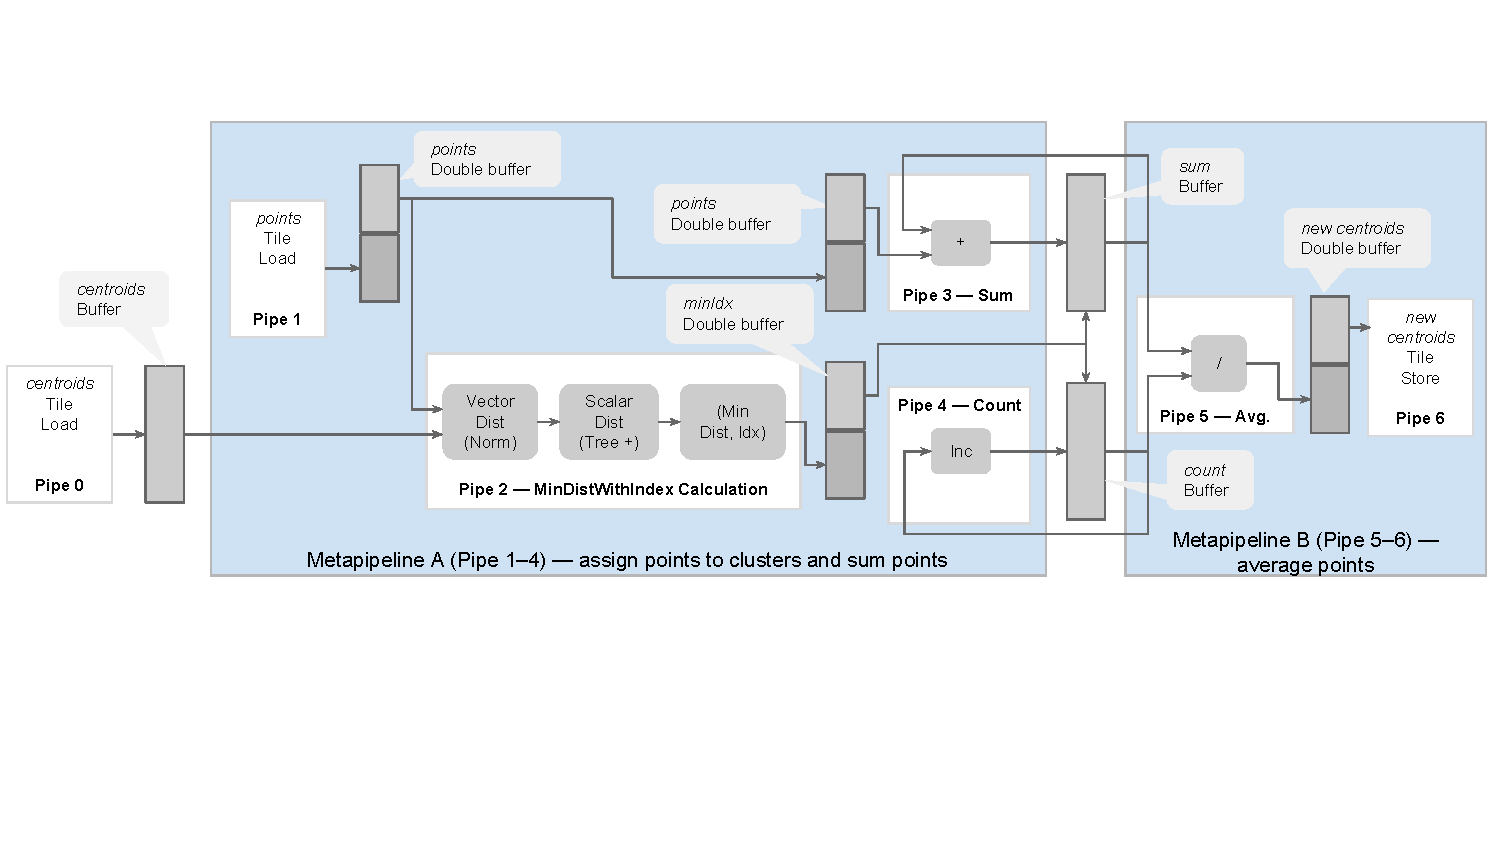
\includegraphics[width=6in]{3-delite/figs/kmeans-blockdiagram.pdf}
\caption{Block diagram of hardware generated for the $k$-means application.}
\label{fig:metapipelining}
\end{figure*}

Figure~\ref{fig:metapipelining} shows a block diagram of the hardware generated for the $k$-means application.
For simplicity, this diagram shows the case where the \emph{centroids} array completely fits on-chip, meaning
we do not tile either the number of clusters \emph{k} or the number of features \emph{d}.

The resulting hardware design contains three sequential steps.
The first step (Pipe~0) preloads the entire \emph{centroids} array into a buffer.
The second step (Metapipeline A) is a coarse-grained pipeline which consists of three stages with buffers to manage communication between the stages.
These three stages directly correspond to the three main sections of the MultiFold (Figure~\ref{fig:kmeans-fused}, line~5) used to sum and count the input points as grouped by their
closest centroid. The first stage (Pipe~1) loads a tile of the \emph{points} array onto the FPGA. Note that this stage was double buffered by the Spatial compiler to
enable hardware prefetching. The second stage (Pipe~2) computes the index of the closest centroid using vector compute blocks and a scalar reduction
tree. The third stage (Pipe~3 and Pipe~4) increments the count for this minimum index and adds the current point to the corresponding location in the
buffer allocated for the \emph{new centroids}.

The third step (Metapipeline B) corresponds with the second outermost parallel pattern in the $k$-means application.
This step streams through the point sums and the centroid counts, dividing each sum by its corresponding count. The resulting new centroids
are then written back to main memory using a tile store unit for further use on the CPU.

Our automatically generated hardware design for the core computation of $k$-means is very similar to the manually optimized design described by Hussain et al.~\cite{hwkmeans}.
While the manual implementation assumes a fixed number of clusters and a small input dataset which can be preloaded onto the FPGA, we use tiling to automatically generate
buffers and tile load units to handle arbitrarily sized data. Like the manual implementation, we automatically parallelize across centroids
and vectorize the point distance calculations. As we see from the $k$-means example, our approach enables us to automatically generate high quality hardware implementations which are comparable to manual designs.
